\documentclass[a4paper]{paper}
\usepackage{amsmath}
\usepackage{pdfpages}
\usepackage{graphicx}
\usepackage{wrapfig}
\usepackage{listings}
\usepackage{multicol}
\usepackage{color}
\usepackage{alltt}
\usepackage{marvosym}
% Style definition file generated by highlight 3.6, http://www.andre-simon.de/ 

% Highlighting theme: Print 

\newcommand{\hlstd}[1]{\textcolor[rgb]{0,0,0}{#1}}
\newcommand{\hlnum}[1]{\textcolor[rgb]{0,0,0}{#1}}
\newcommand{\hlesc}[1]{\textcolor[rgb]{0,0,0}{#1}}
\newcommand{\hlstr}[1]{\textcolor[rgb]{0,0,0}{#1}}
\newcommand{\hlpps}[1]{\textcolor[rgb]{0,0,0}{#1}}
\newcommand{\hlslc}[1]{\textcolor[rgb]{0.4,0.4,0.4}{\it{#1}}}
\newcommand{\hlcom}[1]{\textcolor[rgb]{0.4,0.4,0.4}{\it{#1}}}
\newcommand{\hlppc}[1]{\textcolor[rgb]{0,0,0}{\bf{#1}}}
\newcommand{\hlopt}[1]{\textcolor[rgb]{0,0,0}{\bf{#1}}}
\newcommand{\hllin}[1]{\textcolor[rgb]{0.53,0.53,0.53}{#1}}
\newcommand{\hlkwa}[1]{\textcolor[rgb]{0,0,0}{\bf{#1}}}
\newcommand{\hlkwb}[1]{\textcolor[rgb]{0,0,0}{\bf{#1}}}
\newcommand{\hlkwc}[1]{\textcolor[rgb]{0,0,0}{\bf{#1}}}
\newcommand{\hlkwd}[1]{\textcolor[rgb]{0,0,0}{\bf{#1}}}
\definecolor{bgcolor}{rgb}{1,1,1}


\newcommand{\tabincell}[2]{\begin{tabular}{@{}#1@{}}#2\end{tabular}}
\begin{document}
\tableofcontents
\clearpage
\section{Program architecture}
We use C++/Qt to develop the current plantform, the core of the plantform is a Traffic\_v1 object, which can be described as fig.\ref{UML}

\begin{figure}
\centering
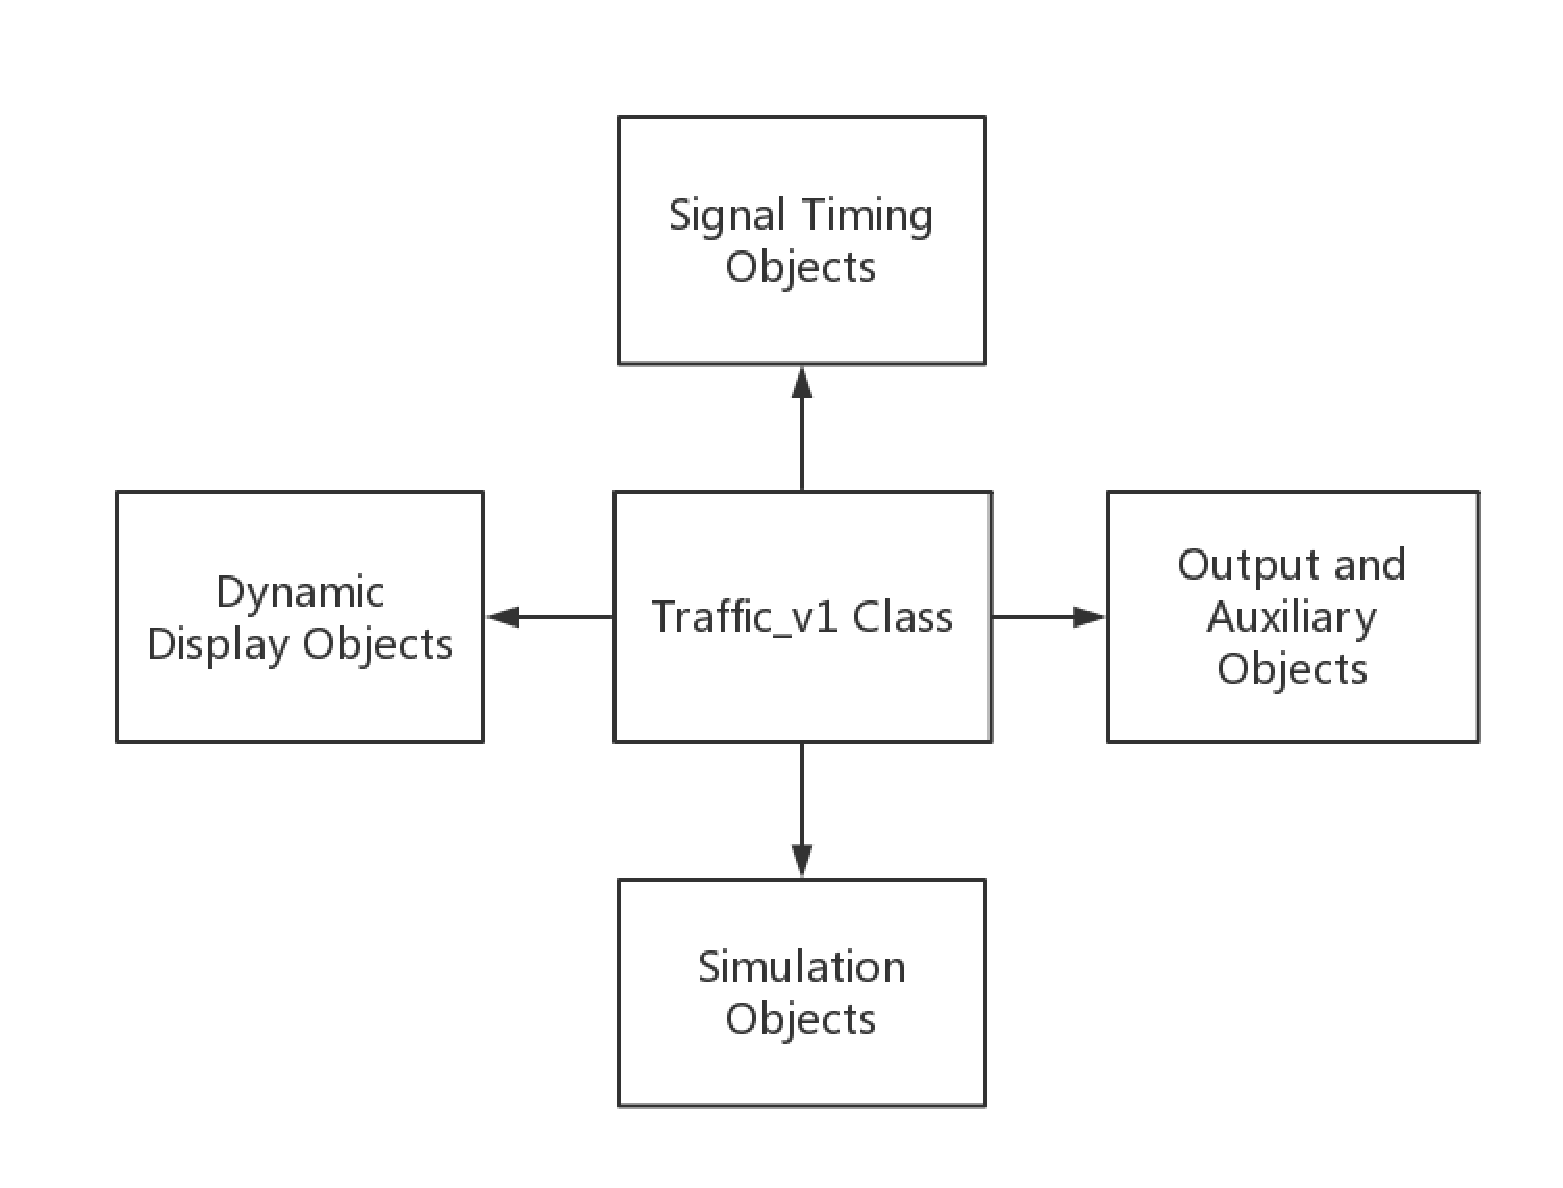
\includegraphics[width=\textwidth]{Diagram.eps}
\caption{The architecture of the Traffic\_v1 class}
\label{UML}
\end{figure}

\subsection{Display module}
These objects are designed for displaying the simulation process dynamicly and controling the simulation process, such as the simulation speed. These objects mainly include the push buttons, labels and the silders.

When a simulation step is put forward, the plantform will refresh the display module to show what has happened during the simulation. The whole function completes the following steps.

\begin{enumerate}
\item Paint the basic elements of the intersection

According to the signal timing module, the painting module will paint the traffic lights. At the same time, it will paint the lanes to the intersection, which is 22.5m in width and 30m in length.

\item Paint the vehicles

In all vehicles in the system, the vehicles heading to the intersection can be controled, while the vehicles leaving the intersection have no need to accept any control strategies, which will be controled by the plantform.

\item Paint the route in the intersection

The plantform dose not deal with the behavior of the vehicle in the intersection, so the trajectory line is used instead of the specific location of the vehicle. When a vehicle runs into the intersection, it is assumed that the retention time of the vehicle turning left is 3s, while the retention time of the vehicle going straight on is 2s and the one of the vehicle turning right is 1s. All of these parameters can be easily changes in the source code.

It can be said that the number of the traces of the trajectory is the degree of the chaos in the intersection, If there are too many crossings, the traffic efficiency may be affected and the danger of the intersection may be increased, this is a main problem of the signal timing.
\end{enumerate}

\subsection{Simulation module}
This is the core module of the plantform, according to the objects used to set the simulation speed, the plantform will emit a trigger signal at an interval of 1ms (for fast speed), 10ms (for medium speed), 100ms (for slow speed) and 1000ms (for debugging). 

When the trigger signal is received, the plantform will follow the instructions in Fig.\ref{int} to perform the relevant operations.

\begin{figure}
\centering
\includegraphics[width=\textwidth]{TimeFlow.png}
\caption{Process of the plantform}
\label{int}
\end{figure}

During the execution process, the process control block determines whether to stop the simulation automatically, according to the stop conditions set by user. Then ,the new vehicls is generated in each lane in accordance with the design of the algorithm to generate the vehicle. After that, the user stratety configuration will apply the user strategy on each of the vehicles according to the mode chosen by user and the type of the vehicle. And the system strategy is responsible for handling the vehivles leaving the intersection and some of the marginal situation of the vehicle, such as entering the intersection. 

All of the strategies mentioned above are changing the acceleration of the vehicle, then during the kinematics simulation, the plantform will calculate the speed and the position of the vehicle according to the vehicle acceleration and the speed.

Eventually, the plantform will handling vehicles that have entered the intersection or are about to leave the area of concern.

In the end, the system repaints the interface, and waits for the arrival of the next trigger signal.

According to the current implementation of the whole plantform, the pressure on the system is appropriate during the 10ms timer interval (medium simulation mode), and the data generated by the system is relatively stable, however, if the timer interval is set to 1ms (i.e. fast simulation mode), some timing problems may occur.

\subsection{Output and auxiliary module}
The main task of this part of the module is to output real-time simulation results, part of which is called when the interface is repainted, and other parts will be called when some specific circumstances occur.

As the simulation progresses, the system creates 4 CSV tables, stored in the folder 'result' under the root directory of the executable directory, and the naming convention for each folder in the folder 'result' is 

\centerline{\textbf{'date+time+simulation mode'}}

And the 4 tables keep a record od different kinds of data.

\begin{enumerate}
\item car.csv

This table keeps a record of the initial speed of the vehicle (init\_velocity), the thoritical time of arrival (thoritical\_time) and the actual time of arriving (act\_time), the thoritical time of arrival is defined as the arrival time when ths vehicle accelerates to maximum speed with maximum acceleration, and maintain a uniform linear motion till enters the intersection. The difference between the thoritical\_time and the act\_time can be described as the time waste driving through this area.

\item stop.csv

This table records the total number of stops per lane at each time and the total number of stops in the system, and the proportion of the total number of vehicles.

\item road.csv

This table records the total number of vehicles leaving a certain lane at each moment and the total number of vehicles leaving the system, and their average

\item stop\_time.csv

This table records the total time of each lane stop at each moment and the total time of parking within the system, as well as the parking time allocated to each vehicle.
\end{enumerate}

Generally speaking, road.csv is used to observe whether the entire simulation process behaves well and the other 3 tables are used to evaluate the merits of the entire strategy.

In addition, the number of stops is determined by whether the speed of the vehicle is below a certain threshold and the stoping time is continuously accumulated as the vehicls stops, besides, the number of stops does not increase during the vehicle's long-term parking.

\subsection{Signal timing module}
The signal timing module meets the user requirements for setting the traffic lights freely. 3 push buttons 'set red behind'; 'set green behind'; 'set yellow behind' are used to set the phase of signal selected behind the black timeline. 

Meanwhile, this interface can be used to set the cycle of the signals. Therefore, by moving the timeline or specify the timeline position, repeatedly selecting the lane to be changed, setting the signal phase. etc, users can set the traffic signals freely.

At the same time, the left interface will prompt the trajectory may exists in the intersection currently (i.e the timeline shows), to prompt the user to avoid the overlap of trajectory, and help users to more reasonable signal timing work.
\subsection{The interface of the plantform}
The interface of the simulation module and the signal timing module are shown as fig.\ref{cap1} and the fig.\ref{cap2}.
\begin{figure}
\centering
\includegraphics[width=\textwidth]{cap1.jpg}
\caption{The interface of the simulation module}
\label{cap1}
\includegraphics[width=\textwidth]{cap2.jpg}
\caption{The interface of the signal timing module}
\label{cap2}
\end{figure} 

The interface of the signal timing module is activated if the user click the 'Edit Traffic Light' Push button. And if the user close the the interface of the signal timing module, the changes made by user will be saved and the interface of the simulation module will be activated.
\clearpage
\section{A brief description of the algorithm}
\subsection{basic assumption and parameters}
Firstly, it is assumed that the physical quantity which is under control directly is the acceleration of the vehicle, while other physical quantities are set because of the theorem given by kinematics, such as 
$$v(t+\Delta_t)=v(t)+a\Delta_t$$
$$x(t+\Delta_t)=x(t)+v(t)\Delta_t+0.5a\Delta_t^2$$ 

However, the acceleration of the vehicle can not be controled precisely, a random noise distributed by normal dirtribution is added into the result given by all of the strategies, especially the ones may operated by human.

As for the speed limit,the platform considers the maximum absolute value of the acceleration of the vehicle is $a_{max}$, which is generally used in the acceleration process and tbe braking process. Also, the maximum speed limit is set to $v_{max}$, while the minimum speed limit is set to $v_{min}$.

No matter which strategy is chosen, if the acceleration given by the strategy is greater than the maximum acceleration $a_{max}$ or less than $-a_{max}$, or the calculated speed is greater than the maximum speed or less than the minimum speed, the program will automatically set these values to the boundary value. When the vehicle has to stop because of the red light, the minimum speed of the vehicle is set to 0, describing the parking behavior which may exist, however, the behavior of reversing is never allowed.

Also, we assume the expected speed of the vehicle, $v_{exp}$, is set to 80\% of the maximum speed limit.

In order to simpliy the simulation process, we assume that during the process of driving, there is no lane changing behavior. This hypothesis is also acceptable in the real life, because of the restrictions imposed by driving habits and traffic laws \& regulations, the vehicle should finish changing lane before enter the traffic junction. Therefore this assumption is reasonable. What's more, just from the perspective of traffic efficiency, lane-changing can only reduce the average efficiency of the traffic, therefore, as the primary inspection of the platform is efficiency, lane-changing situation is not taken into consideration.

Therefore, the car driving in the lane can be described as a queue, i.e. $Q_{in}$

\subsection{The Generation of the vehicles}
It is assumed that the arrival process of the vehicle is approximately a Poisson process, which is limited and adjusted by the following algorithm

Assuming that the intensity of the Poisson process is $\lambda$, the arrival time interval of the vehicle $S_n,S_{n-1}$ can be expressed as 
$$P((S_n-S_{n-1}\le t) = 1 - e^{-\lambda t}$$
Because the simulation time scale is set to 0.1s, the average hourly traffic flow is $$\bar{F}=36000\lambda$$

For the traffic flow in one direction, after the average hourly traffic flow is set by the traffic flow adjustment slider described above, The vehicles in this direction will be generated according to the Poisson process with a specified intensity of $\lambda=\displaystyle{\frac{\bar{F}}{3600}}$, and will be pushed into the pending queue $Q_{pending}$in each direction.

After generating the vehicle, the next step is to consider which lane the vehicle belongs to, and it is assumed that the possibility of the vehicle appearing in each safe lane is same. Firstly, the condition to determine a safe lane is that the distance of last vehicle in the lane and line which the vehicles are generated ($S_{start}$) is greater than the safe distance $S_{safe}$, that is,
$$X_{-1}-S_{start}\le S_{safe}$$

Screening all lanes that meet the situation above in this direction, and place the vehicle in $Q_{pending}$ into one of these lanes randomly, while the position of the vehicle newly generated is set to $S_{start}$.

If there is no lanes suitable for placing the vehicle currently, the vehicles will remain in $Q_{pending}$ and wait for the next simulation session.

The generation of the vehicle is done in the second step of the simulation cycle, just following the process control model.
\subsection{The formation and evacuation of the queue in the intersection}
\label{section:feq}
To describe the phenomenon of queuing aat the intersection, a queue $Q_{block}$ is introduced to each lane towards the intersection. And according to the current signal phase and the length of the queue, all of the control strategies mentioned take these simple algorithm below.
\begin{enumerate}
\item Red Light

If the distance between the first vehicle in $Q_{in}$ and the last vehicle in $Q_{block}$ is less than the control range $S_{control}$, the first vehicle in $Q_{in}$ brake and is expected to stop just behind the last vehicle in $Q_{block}$. The expected distance between these two vehicles is defined as $S_{stop}$, describing the distance between the vehicles in the $Q_{block}$. 

If the $Q_{block}$ is empty and the distance between the first vehicle in $Q_{in}$ and the stopping line is less than $S_{control}$, the first vehicle in $Q_{in}$ brake and is expected to stop just on the stopping line$S_{end}$.

If the first vehicle in the $Q_{in}$is too far that neither of the two above are satisfied, the first vehicle in the $Q_{in}$ is supposed to drive freely.

Also, the vehicles in the $Q_{block}$ should stop and wait until the light truns green.
\item Green Light
distance between the first vehicle in $Q_{in}$ and the last vehicle in $Q_{block}$ (if it exists) should not be less than $S_{safe}$. And a braking is taken if the distance mentioned above is too short.
\end{enumerate}
Therefore, the brief idea of the algorithm above can be described as the fake code below\\ 

\noindent
\ttfamily
\hlstd{}\hllin{01\ }\hlkwa{if\ }\hlstd{}\hlopt{(}\hlstd{Q\textunderscore block}\hlopt{.}\hlstd{}\hlkwd{empty}\hlstd{}\hlopt{())\{}\\
\hllin{02\ }\hlstd{\ }\hlkwa{if\ }\hlstd{}\hlopt{(}\hlstd{Light\ }\hlopt{==\ }\hlstd{Green}\hlopt{)}\\
\hllin{03\ }\hlstd{}\hlstd{\ \ }\hlstd{Q\textunderscore in}\hlopt{.}\hlstd{}\hlkwd{first}\hlstd{}\hlopt{().}\hlstd{}\hlkwd{drive\textunderscore freely}\hlstd{}\hlopt{();}\\
\hllin{04\ }\hlstd{\ }\hlkwa{else}\\
\hllin{05\ }\hlstd{}\hlstd{\ \ }\hlstd{Q\textunderscore in}\hlopt{.}\hlstd{}\hlkwd{first}\hlstd{}\hlopt{().}\hlstd{}\hlkwd{brake\textunderscore to}\hlstd{}\hlopt{(}\hlstd{S\textunderscore end}\hlopt{);}\\
\hllin{06\ }\hlstd{}\hlopt{\}}\\
\hllin{07\ }\hlstd{}\hlkwa{else}\hlstd{}\hlopt{\{}\\
\hllin{08\ }\hlstd{\ }\hlkwa{if}\hlstd{}\hlopt{(}\hlstd{Q\textunderscore block}\hlopt{.}\hlstd{}\hlkwd{last}\hlstd{}\hlopt{().}\hlstd{pos}\hlopt{{-}}\hlstd{Q\textunderscore in}\hlopt{.}\hlstd{}\hlkwd{first}\hlstd{}\hlopt{().}\hlstd{pos}\hlopt{$<$\ }\hlstd{S\textunderscore control}\hlopt{)}\\
\hllin{09\ }\hlstd{}\hlstd{\ \ }\hlstd{Q\textunderscore in}\hlopt{.}\hlstd{}\hlkwd{first}\hlstd{}\hlopt{().}\hlstd{brake\textunderscore to\\
\hllin{10\ }}\hlstd{\ \ }\hlstd{}\hlopt{(}\hlstd{Q\textunderscore block}\hlopt{.}\hlstd{}\hlkwd{last}\hlstd{}\hlopt{().}\hlstd{pos}\hlopt{{-}}\hlstd{S\textunderscore stop}\hlopt{);\ }\\
\hllin{11\ }\hlstd{\ }\hlkwa{else}\\
\hllin{12\ }\hlstd{}\hlstd{\ \ }\hlstd{Q\textunderscore in}\hlopt{.}\hlstd{}\hlkwd{first}\hlstd{}\hlopt{().}\hlstd{}\hlkwd{drive\textunderscore freely}\hlstd{}\hlopt{();}\\
\hllin{13\ }\hlstd{}\hlopt{\}}\hlstd{}\\
\mbox{}
\normalfont
\normalsize


Where the brake\_to(desired\_pos) method means braking to a desired position.

Meanwhile, the growth and the dissipation of the queue $Q_{block}$ follow the method below.

\begin{enumerate}
\item Increase

If the first vehicle in $Q_{in}$ is closer than $S_{stop}$ from the last vehicle in $Q_{block}$ (it is set to $S_{end}$ if the $Q_{block}$ is empty), it is removed from the $Q_{in}$ and pushed into the $Q_{block}$

\item Dissipation

When the traffic light is green, all of the vehicles in the $Q_{block}$ is moving forward at the speed of $v_{dis}$, since the speed is relatively low, the acceleration process and any other phenomenon can be ignored. When the vehicle moves over the stopping lane and enters the intersection, it is removed from the $Q_{block}$
\end{enumerate}
And the method above can be described as the fake code below\\

\noindent
\ttfamily
\hlstd{}\hllin{01\ }\hlkwa{if\ }\hlstd{}\hlopt{(}\hlstd{light\ }\hlopt{==\ }\hlstd{green}\hlopt{)\{}\\
\hllin{02\ }\hlstd{\ Q\textunderscore block}\hlopt{.}\hlstd{}\hlkwd{all\textunderscore move\textunderscore forward}\hlstd{}\hlopt{(}\hlstd{v\textunderscore dis}\hlopt{)}\\
\hllin{03\ }\hlstd{}\hlopt{\}}\\
\hllin{04\ }\hlstd{}\hlkwa{else}\hlstd{}\hlopt{\{}\\
\hllin{05\ }\hlstd{\ }\hlkwa{if}\hlstd{}\hlopt{(!}\hlstd{Q\textunderscore block}\hlopt{.}\hlstd{}\hlkwd{empty}\hlstd{}\hlopt{())\{}\\
\hllin{06\ }\hlstd{}\hlstd{\ \ }\hlstd{}\hlkwa{if}\hlstd{}\hlopt{(}\hlstd{Q\textunderscore block}\hlopt{.}\hlstd{}\hlkwd{last}\hlstd{}\hlopt{().}\hlstd{pos}\hlopt{{-}}\hlstd{Q\textunderscore in}\hlopt{.}\hlstd{}\hlkwd{first}\hlstd{}\hlopt{().}\hlstd{pos\\
\hllin{07\ }}\hlstd{\ \ \ }\hlstd{}\hlopt{$<$\ }\hlstd{S\textunderscore stop}\hlopt{)\{}\\
\hllin{08\ }\hlstd{}\hlstd{\ \ \ }\hlstd{Vehicle\ v}\hlopt{;}\\
\hllin{09\ }\hlstd{}\hlstd{\ \ \ }\hlstd{v}\hlopt{=}\hlstd{Q\textunderscore in}\hlopt{.}\hlstd{}\hlkwd{getfirst}\hlstd{}\hlopt{();}\\
\hllin{10\ }\hlstd{}\hlstd{\ \ \ }\hlstd{Q\textunderscore block}\hlopt{.}\hlstd{}\hlkwd{push}\hlstd{}\hlopt{(}\hlstd{v}\hlopt{);}\\
\hllin{11\ }\hlstd{}\hlstd{\ \ }\hlstd{}\hlopt{\}}\\
\hllin{12\ }\hlstd{\ }\hlopt{\}}\\
\hllin{13\ }\hlstd{\ }\hlkwa{else}\hlstd{}\hlopt{\{}\\
\hllin{14\ }\hlstd{}\hlstd{\ \ }\hlstd{}\hlkwa{if}\hlstd{}\hlopt{(}\hlstd{S\textunderscore end}\hlopt{{-}}\hlstd{Q\textunderscore in}\hlopt{.}\hlstd{}\hlkwd{first}\hlstd{}\hlopt{().}\hlstd{pos}\hlopt{$<$\ }\hlstd{S\textunderscore stop}\hlopt{)\{}\\
\hllin{15\ }\hlstd{}\hlstd{\ \ \ }\hlstd{Vehicle\ v}\hlopt{;}\\
\hllin{16\ }\hlstd{}\hlstd{\ \ \ }\hlstd{v}\hlopt{=}\hlstd{Q\textunderscore in}\hlopt{.}\hlstd{}\hlkwd{getfirst}\hlstd{}\hlopt{();}\\
\hllin{17\ }\hlstd{}\hlstd{\ \ \ }\hlstd{Q\textunderscore block}\hlopt{.}\hlstd{}\hlkwd{push}\hlstd{}\hlopt{(}\hlstd{v}\hlopt{);}\\
\hllin{18\ }\hlstd{}\hlstd{\ \ }\hlstd{}\hlopt{\}}\\
\hllin{19\ }\hlstd{\ }\hlopt{\}}\\
\hllin{20\ }\hlstd{\ }\\
\hllin{21\ }\hlopt{\}}\hlstd{}\\
\mbox{}
\normalfont
\normalsize


All above describe the formation and evacuation of the queue in the intersection and its interaction with other models. The differences caused by the assumption can be ignored. Thanks to this model, it is easy for us to decouple the driving model and the queuing model, which makes it much easier to implement the other algorithm
\subsection{Basic models}
In the description of manual driving and automatic driving vehicle models, the car-following model and free driving model are frequently used models. Therefore, we will describe these models before discussing the control strategies.

\subsubsection{The implementation of the free-driving method}

When there is no speed guidance, a vehicle's driving behavior can be roughly classified into free-driving and car-following, which will be described in this section and the next section. $S_{control}$ is defined as the distance of interaction between vehicles. Thus, the two driving models are chosen according to the rules below.

\begin{enumerate}
\item When the distance to the front vehicle from the vehicle which we are concerned about is less than $S_{control}$, the driving choose the car-following strategy.

\item When the distance is greater than $S_{control}$, the driver choose the free-driving strategy, which means trying to reach the expected speed, $v_{exp}$, during this period, a smaller acceleration may be chosen if the current speed of vehicle is almost the same as $v_{exp}$, while a greater acceleration should be chosen if the current speed is too low, such as the vehicle is stopped.

Also, because some random noise may be introduced to the system, if the speed of the vehicle is higher than $v_{max}$, a minor deceleration should be taken.
\end{enumerate}
\subsubsection{The implementation of the car-following method}
\label{cf}

As mentioned above, when the vehicles is close enough to each other, the car-following method is chosen. In the strategy we used, the commonly used driving psycho-physical model—Wiedemann model is adopted, that is,
$$a_n(t+\Delta_t)=\frac{[\Delta v_{n,n-1}(t)]^2}{2[\Delta x_{n,n-1}(t)-S_{exp}]}+a_{n-1}(t)$$

In the above equation, $S_{exp}$ represents the expected minimum safe-following distance. Since the speed of the vehicle in the intersection may have a big range, $S_{exp}$ should not be a constant. Therefore, according to the regulations on safe distance in Regulation on the Implementation of the Road Traffic Safety Law of the People's Republic of China, we use the linear correlation model of the minimum safe following distance and the speed of the front vehicle, therefore, the $S_{exp}$ can be described like this,
$$S_n(t)=\alpha v_{n-1}(t)+S_{safe}$$
While the $S_{safe}$is the same as the distance between the vehicles in \ref{section:feq}, and the constant $\alpha$ may be set by according to the experience.

Once the distance between the vehicles is less than $S_{exp}$, which means the distance between the vehicles is too short, an emergency brake is taken owing to the specific situation. In most cases, the acceleration of the vehicle is set to $0.5a_{max}$
\subsection{Manual driving model}
\label{section:man}
The plantform provides three models to verify the effectiveness of the platform, and the first model is manual driving model.

As the name of the model indicates, manual driving model is used to describe the behavior of a vehicle driving by human. This model is often used to provide a 'basic' traffic efficiency, while other control strategies are expected to behave better than this simple model.

Firstly, vehicles which are far (greater than $S_{inter}$) from the intersection are taken into consideration. Because they are so far from the intersection, they do not consider the influence of the traffic light. 

Therefore, these vehicles mat take the car-following method or the free-driving method. If a vehicle is the first one in $Q_{in}$, it has to take the the free-driving method.

As for the ones which are closer to the intersection, different method will be chosen to meet the different situation below.

\begin{enumerate}
\item Green traffic light with an empty waiting queue $Q_{block}$

In this situation, the behavior of the vehicles is similar to the behavior described above.

In addition to the behavior mentioned, the remain time of the green light is calculated, if the remaining time is less than $T_{safe}$, the possibility of entering the intersection during the green light may be taken into consider, if it is difficult for the vehicle to pass the stopping line before the light turns red, the vehicle may behave like the traffic light is red.

\item Green traffic light while the  waiting queue $Q_{block}$ is not empty

During this situation, the vehicles discussed may brake or accelerate to set its speed to $v_{dis}$, and try to enter the queue $Q_{block}$, once it enters the $Q_{block}$, it will move with the other vehicles in the queue.

Also, if the remaining time is less than $T_{safe}$, the program may consider slow down the vehicle and prepare to stop. 
\item Red traffic light

In this case, the vehicles discussed will behave just like what we have discussed in \ref{section:feq}
\end{enumerate}

What's more, we focus on portraying the behavior of the first vehicle in the driving queue $Q_{in}$, since the vehicles behind it can be controled easily by car-following method.

Taking all of the situations into consideration. the manual driving model can be abstract as the fake code below.\\
 
\noindent
\ttfamily
\hlstd{}\hllin{01\ }\hlslc{//the\ code\ below\ just\ consider\ the\ vehicle\ v}\\
\hllin{02\ }\hlstd{}\hlkwa{if}\hlstd{}\hlopt{(}\hlstd{S\textunderscore end}\hlopt{{-}}\hlstd{v}\hlopt{.}\hlstd{pos}\hlopt{$>$}\hlstd{S\textunderscore inter}\hlopt{)}\hlstd{}\hlslc{//far\ from\ intersection}\\
\hllin{03\ }\hlstd{}\hlopt{\{}\\
\hllin{04\ }\hlstd{\ }\hlslc{//code\ block\ 1}\\
\hllin{05\ }\hlstd{\ }\hlkwa{if}\hlstd{}\hlopt{(}\hlstd{car}\hlopt{{-}}\hlstd{}\hlkwd{following\textunderscore requirement\textunderscore met}\hlstd{}\hlopt{())}\\
\hllin{06\ }\hlstd{}\hlstd{\ \ }\hlstd{}\hlslc{//the\ car{-}following\ requirement\ is}\hlstd{\ \ }\hlslc{met}\\
\hllin{07\ }\hlstd{}\hlstd{\ \ }\hlstd{}\hlkwd{car\textunderscore following}\hlstd{}\hlopt{();}\\
\hllin{08\ }\hlstd{\ }\hlkwa{else}\\
\hllin{09\ }\hlstd{}\hlstd{\ \ }\hlstd{}\hlslc{//the\ head\ car\ of\ the\ queue\ or}\\
\hllin{10\ }\hlstd{}\hlstd{\ \ }\hlstd{}\hlslc{//the\ car{-}following\ requirement\ isn't\ met}\\
\hllin{11\ }\hlstd{}\hlstd{\ \ }\hlstd{}\hlkwd{free\textunderscore driving}\hlstd{}\hlopt{();}\\
\hllin{12\ }\hlstd{}\hlopt{\}}\\
\hllin{13\ }\hlstd{}\hlkwa{else\ }\hlstd{}\hlslc{//close\ to\ the\ intersection}\\
\hllin{14\ }\hlstd{}\hlopt{\{\ }\\
\hllin{15\ }\hlstd{\ }\hlkwa{if}\hlstd{}\hlopt{(}\hlstd{light}\hlopt{==}\hlstd{red}\hlopt{)}\\
\hllin{16\ }\hlstd{}\hlstd{\ \ }\hlstd{method1}\hlopt{.}\hlstd{}\hlkwd{3}\hlstd{}\hlopt{();}\hlstd{}\hlslc{//the\ method\ mentioned\ in\ 1.3}\\
\hllin{17\ }\hlstd{\ }\hlkwa{else}\\
\hllin{18\ }\hlstd{}\hlstd{\ \ }\hlstd{}\hlkwa{if}\hlstd{}\hlopt{(}\hlstd{Q\textunderscore block}\hlopt{.}\hlstd{}\hlkwd{empty}\hlstd{}\hlopt{())\{}\\
\hllin{19\ }\hlstd{}\hlstd{\ \ \ }\hlstd{}\hlkwa{if}\hlstd{}\hlopt{(}\hlstd{time\textunderscore remain}\hlopt{$>$}\hlstd{T\textunderscore safe}\hlopt{)}\\
\hllin{20\ }\hlstd{}\hlstd{\ \ \ }\hlstd{}\hlslc{//same\ as\ the\ code\ block\ 1}\\
\hllin{21\ }\hlstd{}\hlstd{\ \ \ }\hlstd{}\hlkwa{else\ }\\
\hllin{22\ }\hlstd{}\hlstd{\ \ \ \ }\hlstd{}\hlkwa{if}\hlstd{}\hlopt{(!}\hlstd{}\hlkwd{pass\textunderscore check}\hlstd{}\hlopt{())}\\
\hllin{23\ }\hlstd{}\hlstd{\ \ \ \ }\hlstd{}\hlslc{//same\ as\ the\ red\ light\ case}\\
\hllin{24\ }\hlstd{}\hlstd{\ \ \ }\hlstd{}\hlopt{\}}\\
\hllin{25\ }\hlstd{}\hlstd{\ \ }\hlstd{}\hlkwa{else}\\
\hllin{26\ }\hlstd{}\hlstd{\ \ \ }\hlstd{}\hlkwa{if}\hlstd{}\hlopt{(}\hlstd{time\textunderscore remain}\hlopt{$>$}\hlstd{T\textunderscore safe}\hlopt{)}\\
\hllin{27\ }\hlstd{}\hlstd{\ \ \ }\hlstd{}\hlkwd{acc\textunderscore to\textunderscore speed}\hlstd{}\hlopt{(}\hlstd{v\textunderscore dis}\hlopt{);}\\
\hllin{28\ }\hlstd{}\hlstd{\ \ \ }\hlstd{}\hlkwa{else\ }\\
\hllin{29\ }\hlstd{}\hlstd{\ \ \ \ }\hlstd{}\hlkwa{if}\hlstd{}\hlopt{(!}\hlstd{}\hlkwd{pass\textunderscore check}\hlstd{}\hlopt{())}\\
\hllin{30\ }\hlstd{}\hlstd{\ \ \ \ }\hlstd{}\hlslc{//same\ as\ the\ red\ light\ case}\\
\hllin{31\ }\hlstd{}\hlstd{\ \ \ }\hlstd{}\hlopt{\}}\\
\hllin{32\ }\hlstd{}\hlstd{\ \ }\hlstd{}\\
\hllin{33\ }\hlopt{\}}\hlstd{}\\
\mbox{}
\normalfont
\normalsize


The plantform will traverse the queue $Q_{in}$, and during each iteration, the acceleration of the vehicle in processing will be set according to the model given above.

\subsection{The single-vehicle cooperative speed guidance model}
\label{section:st1}
Applied some changes on the car-following strategy, we designed a cooperative speed guidance model which only takes the influence of the traffic light into consideration.
\subsubsection{Modification about the car-following method}
Firstly, when the distance to the front vehicle from the vehicle which we are concerned about is less than $S_{control}$, the car-following model in chosen. In addition to the basic car-following method, it is changed to the following form when $\Delta x_{n,n-1}(t)\le S_{exp}$ 
$$a_n(t+\Delta_t)=-sgn(\Delta v_{n,n-1}(t))\frac{[\Delta v_{n,n-1}(t)]^2}{2[\Delta x_{n,n-1}(t)-S_{exp}]}+a_{n-1}(t)$$
which means, if the speed of the following vehicle is lower, the strategy will suggest that this vehicle should accelerate.

With this minor modification, some experimental researches show that the changed car-following method works well and can keep a stable distance between the vehicles.

As the fig.\ref{carf} shows, the vehicle following takes the modified car-following method and the front vehicle decelerate with a large random noise. From the figure it can be found that the distance between these two vehicles will be stable near $S_{exp}$, no matter what initial situation is chosen.
\begin{figure}
\centering
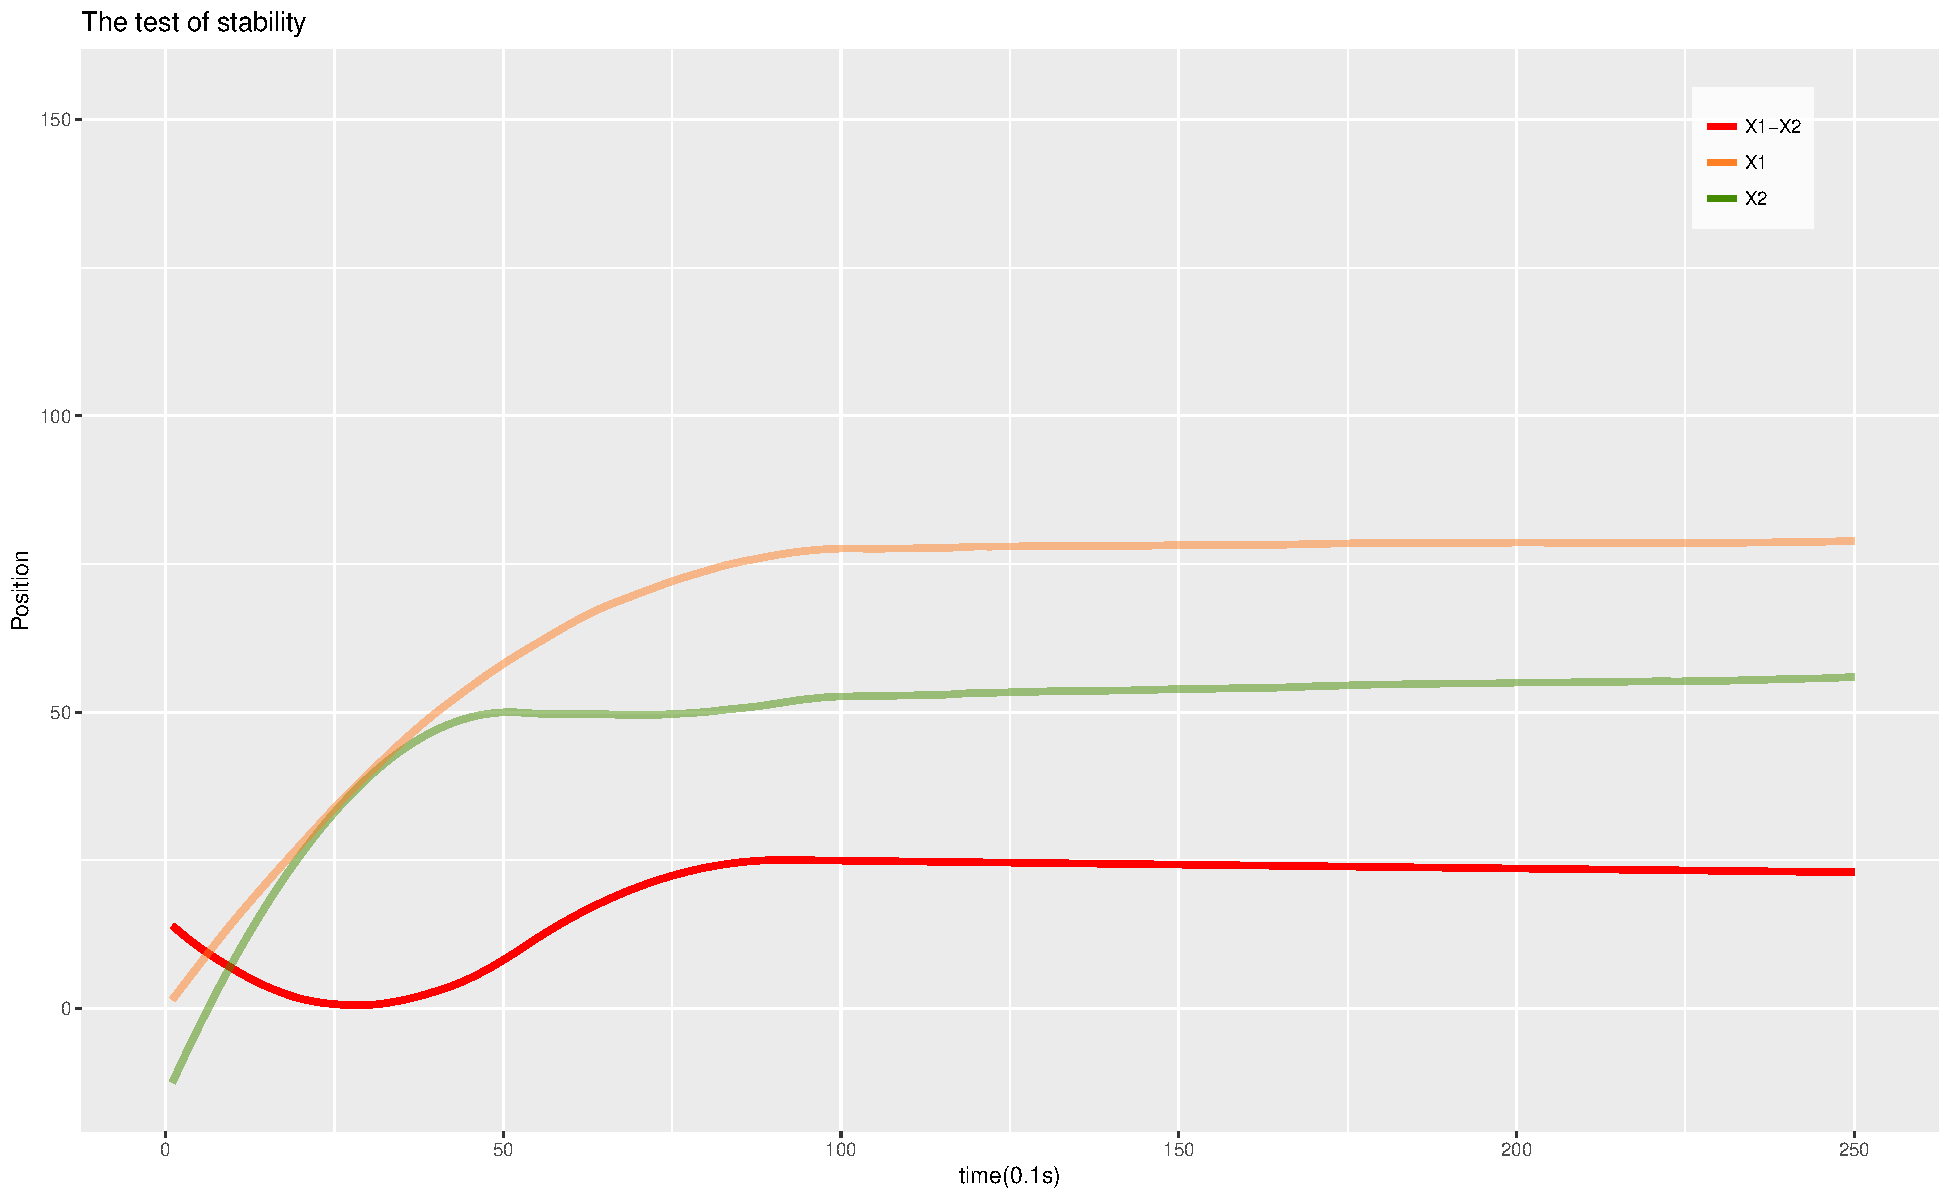
\includegraphics[width=\textwidth]{NearlyGoDie_2.pdf}
\caption{The position of the vehicles and the distance between them}
\label{carf}
\end{figure}
\subsubsection{The cooperative vehicle strategies}
\label{section:tgs}
Besides the chaning on car-following method, the free-driving model is also replaced by the following cooperative vehicle strategy. 

First of all, we define two parameters, the maximum time cost $T_{max}$ is defined as the time cost if the vehicle firstly decelerates at the acceleration of $-a_{max}$ and maintain a uniform linear motion at the speed of $v_{min}$ until it reaches the intersection. Also, the minimum time cost $T_{min}$ is defined as the time cost if the vehicle firstly accelerates at the acceleration of $a_{max}$ and maintain a uniform linear motion at the speed of $v_{max}$ until it reaches the intersection. It is obvious that the actual time cost of a vehicle is less than $T_{max}$ and greater than $T_{min}$, and both the $T_{max}$ and the $T_{min}$ depengs only on the initial speed $v_{init}$ of the vehicle starting from the start line.

Then, the strategy determines the earliest green time $T_G$ in the interval $(T_{min},T_{max}]$ with the accuracy in second. If there is no green time during this interval, a free-driving strategy is applied to the vehicle.

If a proper $T_G$ could be set, an acceleration or a deceleration may be applied to the vehicle to adjust its motion at the aim of reaching the stopping line at the time of $T_G$. During this period, if the vehicle is affected by the preceding vehicle, the car-following model may be applied to the vehicle again.

Meanwhile, the behavior the vehicle takes is similar to the one in the manual driving method.

Generally speaking, this strategy is the optimize version of the car-following model with the consideration of the influence of the traffic light.
\subsection{The multi-vehicle cooperative speed guidance model}
\label{section:st2}
This is a simple connect-vehicle strategy with the communication between the vehicles.

The strategy is operated from the first vehicle in $Q_{in}$ to the last vehicle in $Q_{in}$

First of all, the first vehicle in $Q_{in}$ determine its arrival time $T_G$ according to the method mentioned in section \ref{section:tgs}, and we set the $T_G$ determined by the n-th vehicle in $Q_{in}$ is $T_G^{[n]}$, e.g. the first vehicle determines $T_G^{[1]}$

After chosing the $T_G^{[1]}$, an acceleration or a deceleration may be applied to the vehicle to adjust its motion at the aim of reaching the stopping line at the time of $T_G^{[1]}$, if the $T_G{^[1]}$ does not exist, the vehicle takes an acceleration and then stops at the stopping line.

Then, it is assumed that the [n+1]-th vehicle in $Q_{in}$ can acquire the $T_G^{[n]}$ of the n-th vehicle in $Q_{in}$, including whether it exists.

The [n+1]-th vehicle determins its $T_G^{[n+1]}$according to its $T_{min}$ and $T_{max}$ and make sure that the $T_G^{[n+1]}-T_G^{[n]} \ge 1 \mathrm{second}$, owing to the fact that the following vehicle is supposed to arrive later than the preceding vehicle.

If the $T_G^{[n]}$ does not exist, $T_G^{[n]+1}$ should be set freely, only depends on the $T_{max}$ and the $T_{min}$ of the vehicle.

Then the acceleration of the [n+1]-th vehicle is set according to the expected time of arrival. The strategy then goes for the following vehicles.

Since the expected time of arrival is carefully designed to make sure that the following vehicle always arrives the stopping line later than the preceding vehicle, even the vehicles which do not have an expected arrival time will take an acceleration, the probability of the rear-ending is minor, a rear-ending will be solve by some simple emergency settings. 
\subsection{The processing of the strategies and the combination of the strategies}
\subsubsection{Single strategy simulation}
The plantform treats the strategies as an iteration from the last vehicle in the $Q_{in}$ to the first one in that, for the reason that the following vehicles may acquire the acceleration of the preceding car which should be fixed until the acceleration is set according to the strategy chosen by user. 

Therefore, if only a specific strategy is chosen, the program behaves like a loop from the last to the first of $Q_{in}$.

\subsubsection{Combination of the strategies}
Only the combination of the manual driving vehicle and the speed guidance models are concerned about, therefore, the plantform only include two kinds of combination simulation, which is the combination between the manual driving vehicle(mentioned in \ref{section:man}) and the single-vehicle cooperative speed guidance model (mentioned in \ref{section:st1}); and the combination between the manual driving vehicle and the multi-vehicle cooperative speed guidence model (mentioned in \ref{section:st2})

During the vehicle generating step, the control strategy of the vehicle is set by random method according to the type of combination and the ratio set by user.

After generate the type of the control strategy, the user-strategy step of the simulation set the acceleration of the vehicle using the strategy it has. It is assmued that if a vehicle using multi-vehicle cooperative speed guidence model is following a manual driving vehicle, the expected arrival time of the manual driving vehicle $T_G$ does not exist, therefore, the speed guidence model could set its expected arrival time $T_G$ freely.

\subsection{Add on algorithms}
Besides this, some add on algorithm is added to treat some accidents may happen accidentally. And the implementations of these specific algorithms may be found in the code of the plantform.
\end{document}